\section{Content Creation}\label{section:content-creation}

This section describes the usage of \tool from a teacher's perspective. It illustrates the steps that have to be taken in order to create programming assignments that fit the needs of a certain course or course module.

\begin{figure}
\centering
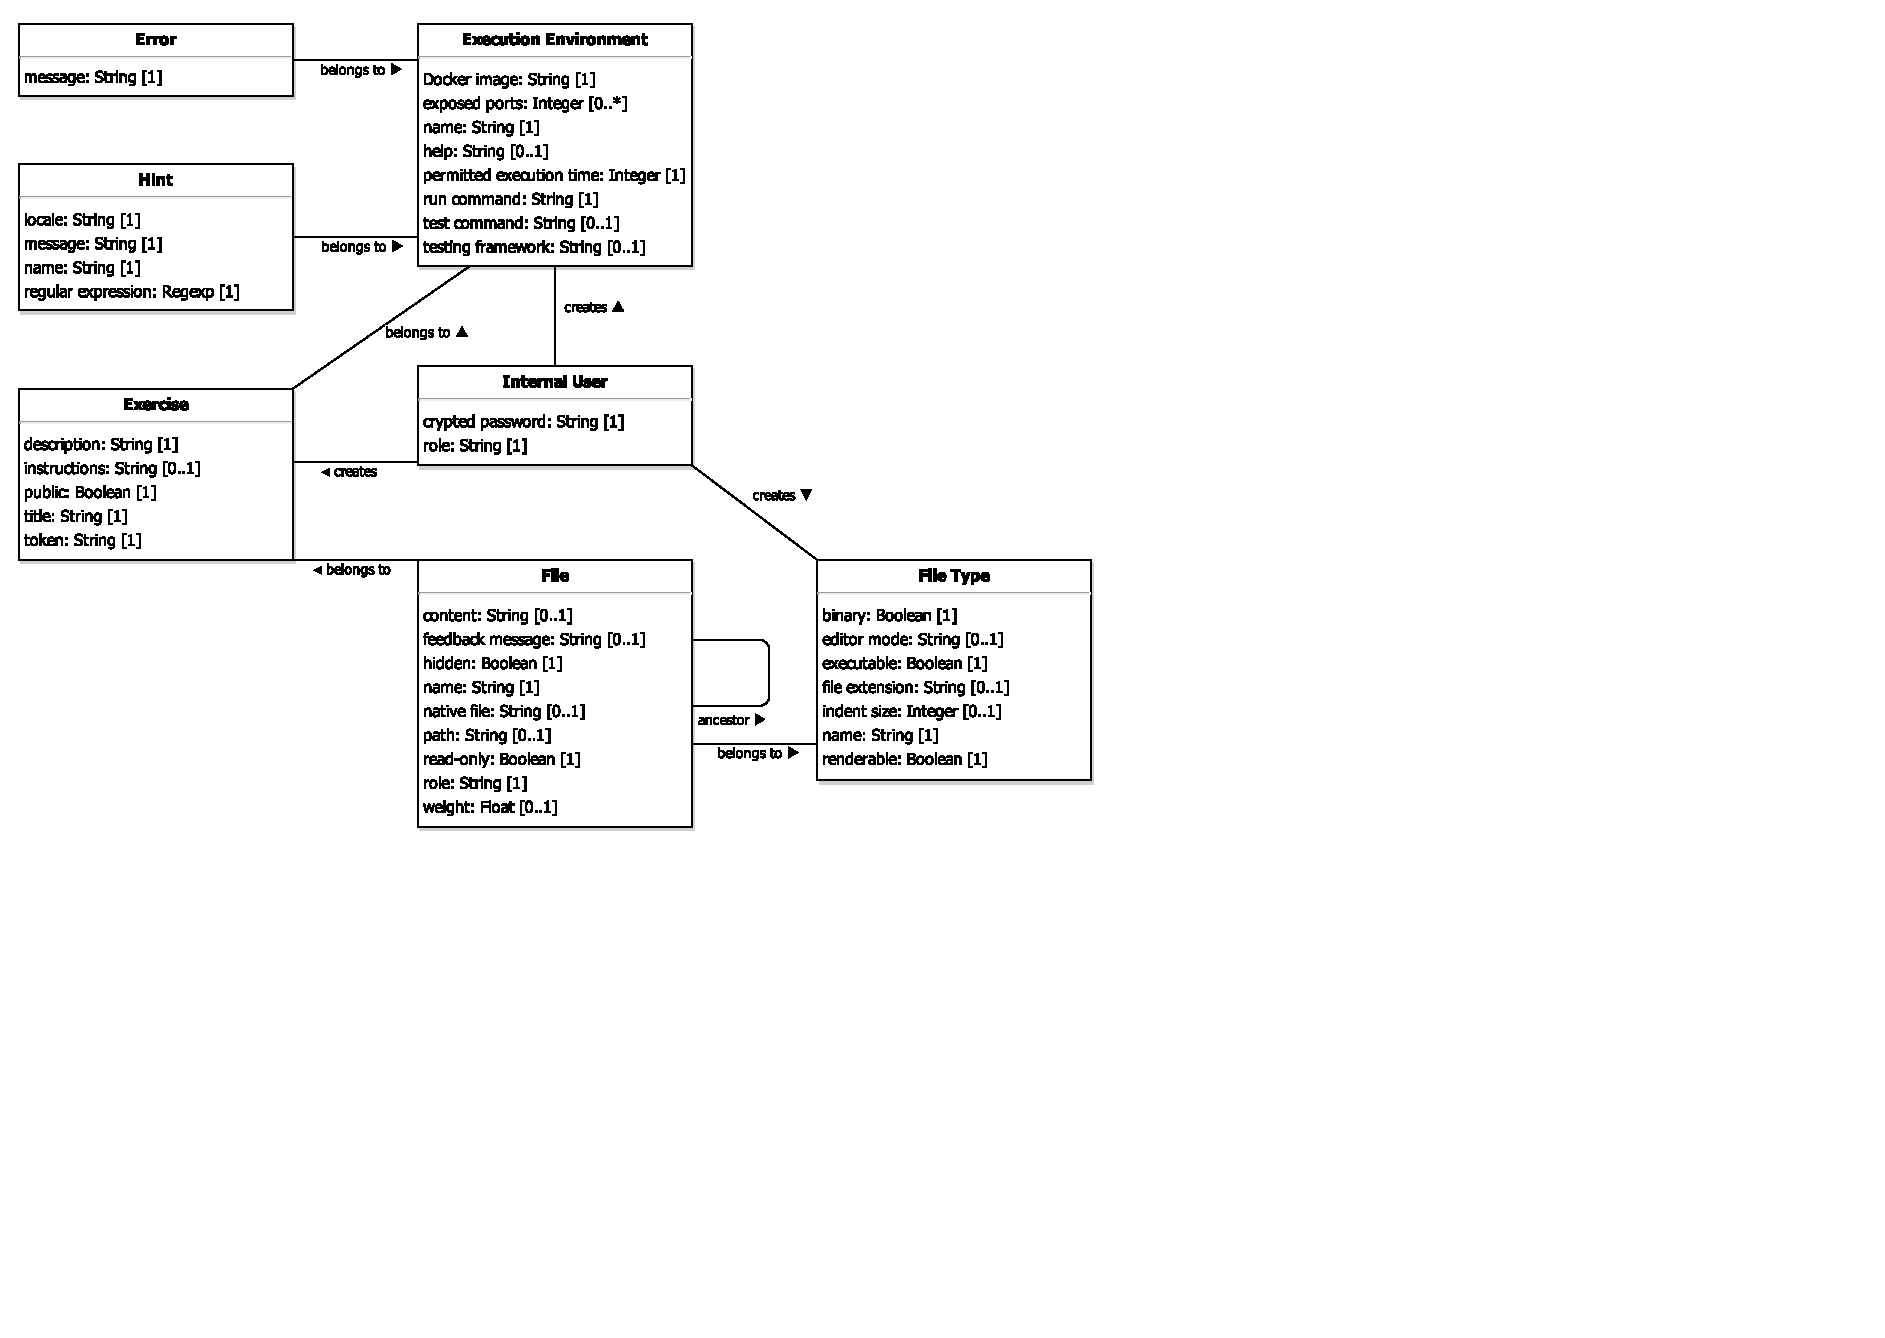
\includegraphics[clip=true, trim=0.3cm 8.1cm 13.2cm 0.3cm, width=\textwidth]{images/domain-model2.pdf}
\caption{\gls{uml} Class Diagram Presenting an Excerpt from the Application’s Domain Model}
\label{figure:domain-model2}
\end{figure}

Figure~\ref{figure:domain-model2} depicts an excerpt from \tool's domain model, as presented in Section~\ref{section:domain-model}, which focuses on entities that are relevant for content creation.

\begin{figure}
\centering
\includegraphics[clip=true, trim=0.1cm 14.6cm 8.8cm 0.1cm, width=\textwidth]{images/content-creation.pdf}
\caption{Steps of the Content Creation Process}
\label{figure:content-creation}
\end{figure}

In order to create content, teachers have to sign in to \tool's administration back-end (see Figure~\ref{figure:administration}) using their email address and password. Usually, their content creation process involves the steps presented in Figure~\ref{figure:content-creation}. Steps depicted using solid lines are mandatory. Steps depicted using dashed lines are optional or apply only once per execution environment.

\begin{figure}
\centering
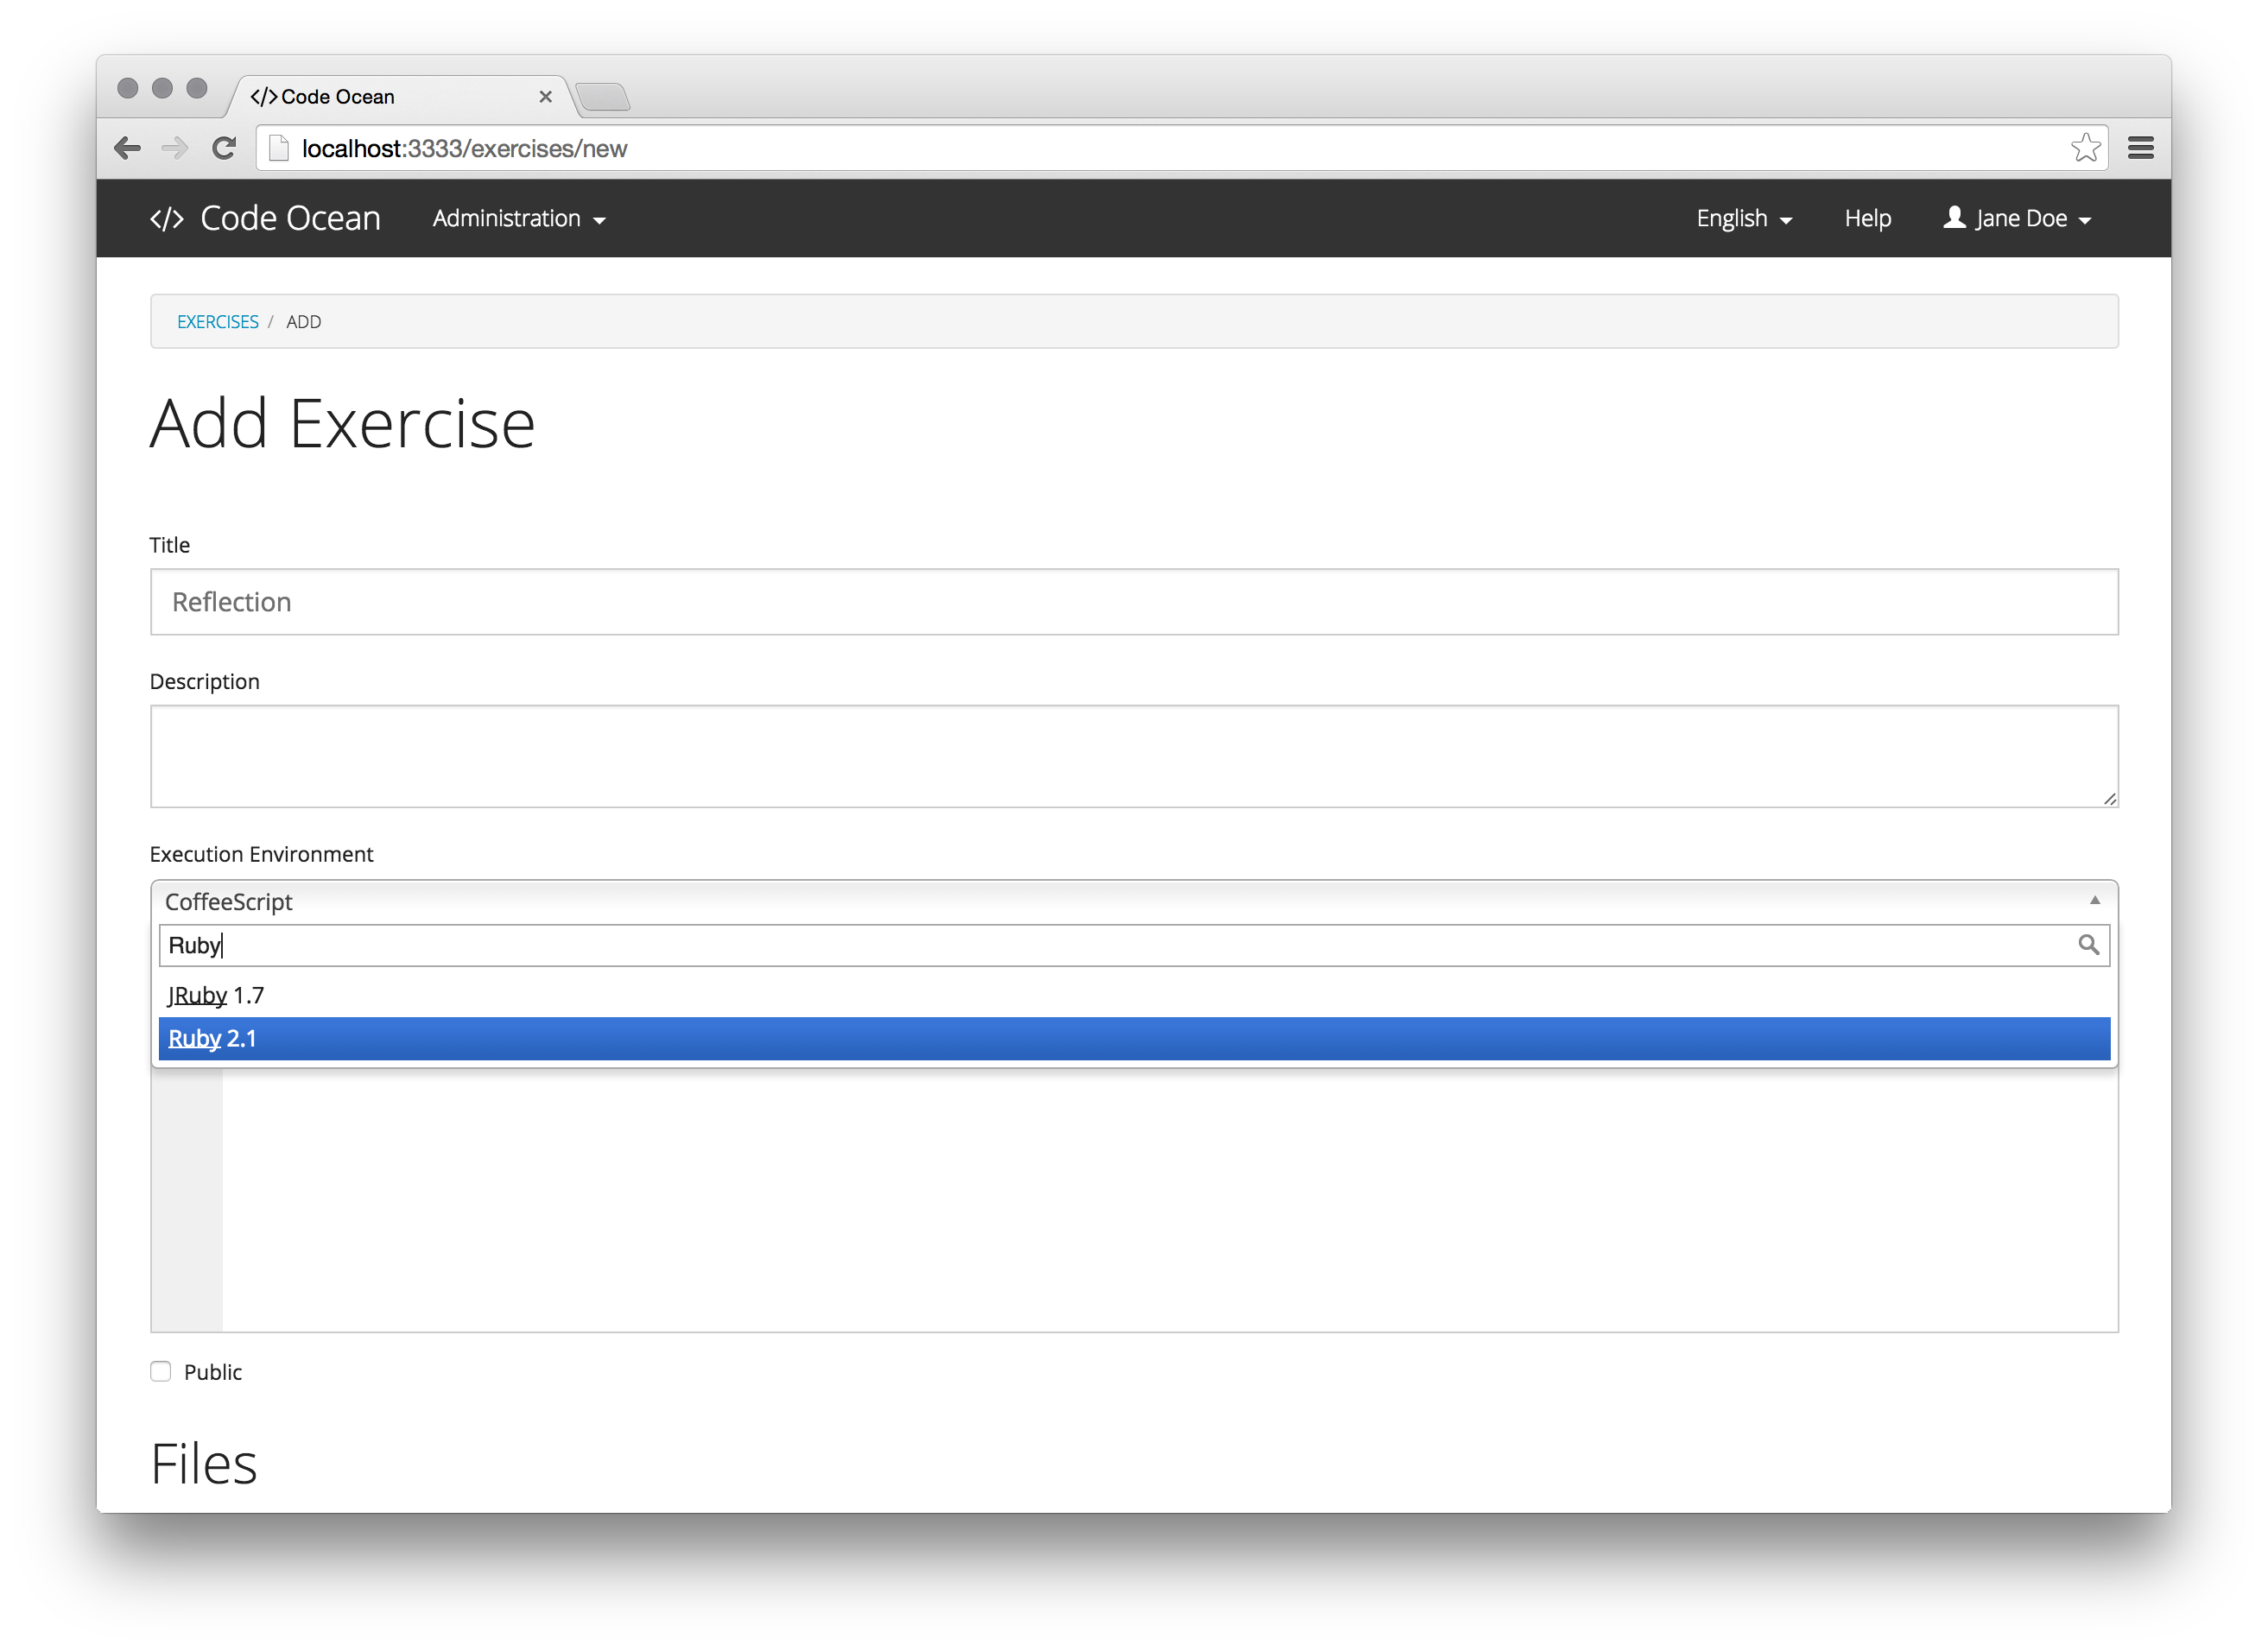
\includegraphics[width=\textwidth]{images/administration.png}
\vspace{-1cm}
\caption{Administration Back-End}
\label{figure:administration}
\end{figure}

\subsection{Execution Environment}

The first step to create content for a new course is to create a qualified execution environment.

The core of an execution environment is its Docker image. In order to create a new execution environment, an instructor can either choose to reuse a Docker image that is already known to \tool through an existing execution environment or can set up a new one. A new Docker image is specified using its identifier, such as \emph{hklement/ubuntu-ruby:2.1.5}, which is composed of the repository name and an optional tag. Images are expected to be publicly available at Docker Hub, so that \tool can download them. An instructor may pick an arbitrary Docker image that is published at Docker Hub or prepare a custom one by hand.

As introduced in Section~\ref{section:code-execution1}, Dockerfiles provide a useful means for the reproducible creation of Docker images. Since Dockerfiles can build up on existing Docker images, the instructor may decide to reuse an existent image as a foundation. In order to foster the reusability of execution environments that \tool already provides, their corresponding Docker images and Dockerfiles are publicly available. Docker images are hosted at Docker Hub\foo{https://hub.docker.com/u/hklement/}, whereas Dockerfiles can be found at GitHub\foo{https://github.com/hklement/dockerfiles}.

\begin{listing}
\inputminted[frame=lines]{Dockerfile}{listings/Dockerfile-jruby}
\vspace{-0.33cm}
\caption{Dockerfile Describing a JRuby Environment}
\label{listing:dockerfile-jruby}
\end{listing}

Listing~\ref{listing:dockerfile-jruby} depicts a Dockerfile describing a JRuby\foo{http://jruby.org/} environment. Since JRuby requires a \gls{jvm}, the Dockerfile is based on \tool's Java Docker image that provides the required dependencies.

Apart from a Docker image, the teacher has to specify a few other attributes when creating a new execution environment. These attributes include the permitted execution time for students' code submissions, a testing framework, as well as the commands for running the student's main program and the associated tests. An extensive list of execution environments' properties is presented in Section~\ref{section:domain-model}.

\begin{listing}
\inputminted[frame=lines]{text}{listings/test-command.txt}
\vspace{-0.33cm}
\caption{RSpec-specific Test Command}
\label{listing:test-command}
\end{listing}

The commands for running student code and for executing tests usually expect a filename. For that reason, both commands can contain a placeholder that is replaced by an actual filename before invocation. For instance, the command depicted in Listing~\ref{listing:test-command} is appropriate for assessing a student's submission using RSpec. To run a test, the command's \emph{filename} placeholder is replaced by the actual filename of the test file.

In order to inspect her newly created execution environment, the creator can either utilize a Docker container on her local machine or use a simple shell provided by \tool. This way, tests and sanity checks can be performed without being limited to the application's conventional development workflow.

\subsection{Exercise}

A new programming exercise can either be created from scratch or by cloning and adjusting an existing assignment. The second option allows to reduce the considerable effort for implementing automatically gradable exercises~\cite{pieterse2013automated} by reusing parts of similar ones.

Consider the example of the Fibonacci sequence~\cite{koshy2011fibonacci}, a programming problem that is commonly used to teach the basics of recursion. The definition of the Fibonacci sequence is depicted in Figure~\ref{figure:fibonacci-sequence}. In order to create an exercise based on the Fibonacci sequence, an instructor has to specify title, description, and instructions, and has to create a number of files.

\begin{figure}
\begin{equation}
fibonacci(n) =
\begin{cases}
n & \text{if } n \leq 1 \\
fibonacci(n - 1) + fibonacci(n - 2) & \text{otherwise}
\end{cases}
\end{equation}
\caption{Definition of the Fibonacci Sequence}
\label{figure:fibonacci-sequence}
\end{figure}

As emphasized in Section~\ref{section:assessment1}, exercise instructions should be provided in a detailed, unambiguous fashion. In this regard, Vihavainen et al.~\cite{vihavainen2012multi} recommend to make instructions as informative as possible and to include exemplary inputs with their expected outputs since this helps learners to confirm that they are proceeding into the right direction.

To enable a continuous workflow, all files associated to an exercise can be created within the exercise form. For an efficient workflow, instructors should prepare and test their exercises using their favorite tools on a local machine or in a Docker container. Afterwards, the completed exercise files can be uploaded. Besides a file's content, several other properties, including name, file type, and role, have to be defined. A complete list of properties can be found in Section~\ref{section:domain-model}.

\begin{listing}
\inputminted[frame=lines]{rb}{listings/exercise.rb}
\vspace{-0.33cm}
\caption{Exemplary Exercise Skeleton}
\label{listing:exercise}
\end{listing}

\tool does not dictate a certain exercise structure. However, a main file that constitutes the starting point for students' implementation should be provided. Based on her learners' level of knowledge, an instructor may choose to provide a program foundation ranging from a blank file to an extensive code skeleton, annotated with comments. A reasonable code skeleton for a Ruby-based Fibonacci sequence exercise is presented in Listing~\ref{listing:exercise}.

In order to create the basis for automated assessment, one or more test files containing test cases based on the exercise's execution environment's testing framework have to be defined. As discussed in Section~\ref{section:assessment2}, in order to increase the value of automated assessment for novice programmers, a helpful feedback message, which is presented to the learner when tests fail, has to be provided for every test file. Such a message might explain what went wrong and could provide hints on how to adjust the code.

By assigning different weights to test files, teachers can control the individual scores awarded for passing tests. Depending on their learners' capabilities, weighting might be used to increase or decrease the significance of challenging problem aspects for the final grade.

Tests should be defined in a manner that enables students to progress in small steps. In terms of the Fibonacci sequence example, the most basic test case might validate the existence of a \mintinline{rb}{fibonacci} method that has an arity of one. Further test cases might validate that the method returns the expected values, behaves correctly in edge cases, and works recursively.

\begin{listing}
\inputminted[frame=lines]{rb}{listings/exercise_spec_1.rb}
\vspace{-0.33cm}
\caption{RSpec Test Validating the \mintinline{rb}{fibonacci} Method’s Existence and Arity}
\label{listing:fibonacci-spec1}
\end{listing}

\begin{listing}
\inputminted[frame=lines]{rb}{listings/exercise_spec_2.rb}
\vspace{-0.33cm}
\caption{RSpec Test Validating the \mintinline{rb}{fibonacci} Method’s Recursiveness}
\label{listing:fibonacci-spec2}
\end{listing}

RSpec-based tests corresponding to two of these test cases are depicted in Listings~\ref{listing:fibonacci-spec1} and~\ref{listing:fibonacci-spec2}. The first test uses the metaprogramming capabilities of the \mintinline{rb}{method} method, defined by Ruby's \mintinline{rb}{Kernel}\foo{http://www.ruby-doc.org/core-2.1.5/Kernel.html} module, to check the existence and arity of the \mintinline{rb}{fibonacci} method. Testing the method's recursiveness works by observing the number of times it is invoked during test execution.

Please note that tests like these are enabled by the ability to use a Ruby-specific testing framework. In contrast, a more universal yet more limited assessment approach, such as \gls{io}-based assessment, would not permit to obtain the insights required for these tests.

\subsection{Testing Framework Adapter}

The instructor is flexible in her choice of a testing framework to use for the specification of automatically assessable assignments. However, if the chosen testing framework is not supported by \tool yet, a testing framework adapter has to be provided that can extract key figures from the framework's textual output (see Section~\ref{section:assessment3}).

In order to keep the effort for preparing such an adapter at a minimum, \tool supplies a generator for testing framework adapters, which integrates into Rails' built-in generator infrastructure.

\begin{listing}
\inputminted[frame=lines]{sh}{listings/generator-invocation.sh}
\vspace{-0.33cm}
\caption{Exemplary Generator Invocation for Generating a Testing Framework Adapter for the Jasmine Testing Framework}
\label{listing:generator-invocation}
\end{listing}

The said generator can be invoked as depicted in Listing~\ref{listing:generator-invocation} using the example of the testing framework Jasmine\foo{http://jasmine.github.io/}. Besides a skeleton for a testing framework adapter, a second one for a corresponding unit test is generated. By completing both skeletons in a way that meaningful tests are defined and that these tests pass, the instructor can ensure to contribute a working piece of software.

After a new testing framework adapter has been prepared and integrated into the application, a newly supported testing framework appears in \tool's administration interface.

\subsection{Hints}

As addressed in Section~\ref{section:hint-generation1}, teachers can supply their students with helpful hints regarding mistakes they make.

If an instructor has created a new execution environment, it has no associated hints yet. In order to change this, hints can either be provided in advance, based on the instructor's experience and expectations, or on demand, based on errors that occurred most during the execution of learners' code.

Just as the other resources, hints are created using the administration back-end. As discussed in Section~\ref{section:hint-generation2}, the teacher has to provide a regular expression and a helpful message for every hint.
